% !TeX encoding = UTF-8 Unicode

%%%%%%%%%%%%%%%%%%%%%%%%%%%%%%%%%%%%%%%%%%%%%%%%%%%%%%%%%%
%
%     Контрпримеры
%
%%%%%%%%%%%%%%%%%%%%%%%%%%%%%%%%%%%%%%%%%%%%%%%%%%%%%%%%%%

\chapter{Контрпримеры}
\label{chap:Counterexamples}

%\hfill
\begin{flushright}
\begin{minipage}{0.4\textwidth}
Теории приходят и уходят,\\ а~примеры остаются.
\begin{flushright}
\emph{И.\,М.~Гельфанд}
\end{flushright}
\end{minipage}
\end{flushright}
\bigskip

%\hfill
%\begin{minipage}{0.55\textwidth}
%Трудно заслужить благодарность за открытие того, как наилучшим способом обойтись без некоторых признанных, но чрезмерно сложных концепций.
%\begin{flushright}
%Э.\,В.~Дейкстра
%\end{flushright}
%\end{minipage}

Целью настоящей главы является ответ на следующий вопрос.
Можно~ли, зная только комбинаторные свойства 
%(однозначно определяемые матрицей инциденций вер\-шин-ги\-пер\-гра\-ней) 
многогранника, отделить NP"=трудные задачи от полиномиально разрешимых?
% (в рамках современных представлений о сложности задач)?
В~разное время в~качестве таких ключевых характеристик сложности рассматривались: число вершин многогранника, число его гиперграней, диаметр и~кликовое число графа, число прямоугольного покрытия матрицы инциденций вершин"=гиперграней.

В первом и втором разделах данной главы приводятся примеры семейств многогранников,
для которых значения упомянутых выше характеристик существенно отличаются от реальной вычислительной сложности (см. замечание~\ref{rem:RealComplexity}) соответствующих оптимизационных задач.
В третьем разделе приводятся примеры двух линейных задач комбинаторной оптимизации, 
многогранники которых комбинаторно эквивалентны 
и~длины двоичной записи координат вершин этих многогранников одинаковы. 
При этом первая задача разрешима за~полиномиальное время, 
а~вторая задача NP"~трудна.

\section{Простые примеры}
\label{sec:SimpleCounterexamples}

\subsection{Число вершин}

Предположим, что вершины многогранника $X$ могут быть эффективно перечислены. Тогда задача линейной оптимизации на $X$ может быть решена с помощью простого перебора. Откуда следует, что число вершин многогранника может служить верхней оценкой сложности соответствующей оптимизационной задачи. То, насколько далекой от реальности может быть эта оценка, иллюстрирует следующий, хорошо известный факт. Задача оптимизации на множестве вершин куба $\{0,1\}^d$ может быть решена за $d$ шагов, тогда как число вершин равно~$2^d$.

\subsection{Число гиперграней}

Так как задача линейного программирования полиномиально разрешима~\cite{Khachiyan:1979,Karmarkar:1984}, то число гиперграней (точнее, полином от него и размерности) многогранника может служить верхней оценкой сложности.
Примером, когда эта оценка оказывается слишком грубой, может служить перестановочный многогранник $\Perm(n)$, число вершин которого равно $n!$, число гиперграней равно $2^n-2$, а задача линейной оптимизации на $\Perm(n)$ имеет сложность порядка $\Theta(n \log n)$.
Заметим, что сложность расширения этого многогранника тоже равна $\Theta(n \log n)$~\cite{Goemans:2015}.

\subsection{Диаметр графа}

До сих пор популярностью пользуются оценки диаметров графов различных семейств многогранников (см. обзор в разделе~\ref{sec:diameter}). Утверждается, что решение полиномиальной гипотезы Хирша окажет влияние на оценки сложности задач линейного программирования~\cite{Santos:2013}. Несостоятельность этого утверждения иллюстрируется следующим фактом. Предположим, что нам известно H-описание \(\Set{\bm{x} \in \R^d \given A\bm{x} \le \bm{b}}\) некоторого (как угодно сложного) многогранника $P$. (Без этого предположения оценки диаметра теряют практический смысл, так как предполагают использование алгоритмов типа симплекс"=метода.) Тогда, увеличив размерность пространства на единицу, можно легко построить пирамиду $Q$ над $P$ 
(не уменьшая общности, предполагаем, что $\bm{0} \in P$):% Например,
\begin{equation}
\label{eq:PyrQ}
Q = \Set*{(\bm{x}, y) \in \R^{d+1} \given A\bm{x} + \bm{b} y \le \bm{b}, \ y \ge 0}.
\end{equation}
Тогда задача линейной оптимизации на $P$ элементарно сводится к оптимизации на $Q$.
С другой стороны, диаметр графа любой пирамиды не превышает двух, так как вершина (апекс) пирамиды непосредственно соединена ребрами со всеми вершинами основания.

В этой связи заметим также, что за счет небольшого шевеления вектора коэффициентов $\bm{b}$ при переменной $y$ в формуле~\eqref{eq:PyrQ} можно прийти к следующему выводу. Любой простой $d$"~многогранник с $n$ гипергранями может быть реализован как гипергрань (или ортогональная проекция) простого $(d+1)$"~многогранника $Q'$ с $n+1$ гипергранями такого, что диаметр $Q'$ не превышает $2(n - d)$~\cite{Lee:1991}.
Этот вывод также, как и предыдущий пример указывает на бесполезность оценок диаметра графа многогранника с точки зрения практики.
Обратим также особое внимание на то, что как пирамида $Q$, так и многогранник $Q'$ являются расширениями многогранника $P$.


\subsection{Кликовое число графа}
\label{subsec:CliqueCounterex}

Оказывается, несостоятельность использования кликового числа графа многогранника для характеризации сложности задач тоже может быть продемонстрирована с помощью расширения многогранника.
Вспомним, что расширением любого многогранника на $n+1$ вершинах является симплекс $\Delta_n$. 

\begin{prop}[\cite{Maksimenko:2016complexity}]
	\label{th:simplex}
	Для любого симплекса $\Delta_d\subset\R^d$ существует 
	его расширенная формулировка $Q_{d+1}\subset\R^{d+1}$, для которой кликовое число $\omega(Q_{d+1}) = 2$.
\end{prop}

\begin{proof}
	Воспользуемся тем фактом, что любые два $d$"~мерных симплекса аффинно эквивалентны друг другу.
	Поэтому далее рассматриваем только наиболее удобный симплекс
	\[
	\Delta_{d-1} = \R_+^d \cap H,
	\]
	являющийся пересечением неотрицательного ортанта $\R_+^d$ и~гиперплоскости
	\[
	H = \left\{\bm{x}=(x_1, \dots, x_d) \in \R^d \mid \bm{1}^T \bm{x} = 1\right\}.
	\]
	
	Мы построим расширенную формулировку $Q_d \subset \R^d$ 
	так, что её ортогональная проекция на $H$ совпадает с $\Delta_{d-1}$.
	Для случая $d=3$ этапы построения изображены на рис.~\ref{fig:1}.
	В общем случае конструкция очень похожа на операцию склейки двух простых многогранников (в частности, двух гиперкубов), описанную в~\cite{Barnette:1969}.
	
	\begin{figure}
		\centering
		\begin{minipage}{0.2\textwidth}
	\centering
	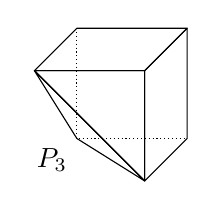
\begin{tikzpicture}[scale=1.4, line join = round]
	\coordinate (1) at (1,0,0);
	\coordinate (2) at (0,0,-1);
	\coordinate (3) at (1,0,-1);
	\coordinate (4) at (0,1,0);
	\coordinate (5) at (1,1,0);
	\coordinate (6) at (0,1,-1);
	\coordinate (7) at (1,1,-1);
	\draw[densely dotted] (6) -- (2) -- (3);
	\draw (4) -- (5) -- (7) -- (6) -- cycle; % верх
	\draw (1) -- (3) -- (7) -- (5) -- cycle; % право
	\draw (1) -- (4) -- (5) -- cycle; % перед
	\draw (1) -- (2) -- (4) -- cycle; % срез
	\draw (2) node[below left] {$P_3$};
	\end{tikzpicture}
\end{minipage}
\hfill
$\Longrightarrow$
\hfill
\begin{minipage}{0.25\textwidth}
	\centering
	\begin{tikzpicture}[scale=1.2, line join = round]
	%cnode/.style={inner sep = 0mm, minimum size = 2pt, circle, text centered,
	%		draw=black, thick, fill=black}]
	\coordinate (x) at (1, 0, 0);
	\coordinate (y) at (0, 0, 1);
	\coordinate (z) at (0,-1, 0); 
	
	\coordinate (a) at ($-1*(x)$);
	\coordinate (b) at (x);
	\coordinate (c) at (${sqrt(3)}*(y)$); %1.7321016);
	%\coordinate (c) at (0, 0, 1.7321016);
	\coordinate (d) at ($0.5*(a) + 0.5*(b) + sin(60)*(z)$);
	\coordinate (e) at ($0.5*(b) + 0.5*(c) + sin(60)*(z)$);
	\coordinate (f) at ($0.5*(a) + 0.5*(c) + sin(60)*(z)$);
	\coordinate (g) at ($1/3*(a) + 1/3*(b) + 1/3*(c) + 1/sin(60)*(z)$);
	
	\draw[densely dotted] (a) -- (d) -- (b) -- cycle (d) -- (g);
	\draw (b) -- (e) -- (c) -- cycle;
	\draw (c) -- (f) -- (a) -- cycle;
	\draw (c) -- (e) -- (g) -- (f) -- cycle; % Перед
	\draw (a) -- (b) -- (c) -- cycle; % Bottom
	\draw (e) +(1ex, 0) node[right] {$Q^-$};
	
	\begin{scope}[yshift = 3mm]
	\coordinate (x) at (1, 0, 0);
	\coordinate (y) at (0, 0, 1);
	\coordinate (z) at ( 0, 1, 0); 
	
	\coordinate (a) at ($-1*(x)$);
	\coordinate (b) at (x);
	\coordinate (c) at (${sqrt(3)}*(y)$); %1.7321016);
	%\coordinate (c) at (0, 0, 1.7321016);
	\coordinate (d) at ($0.5*(a) + 0.5*(b) + sin(60)*(z)$);
	\coordinate (e) at ($0.5*(b) + 0.5*(c) + sin(60)*(z)$);
	\coordinate (f) at ($0.5*(a) + 0.5*(c) + sin(60)*(z)$);
	\coordinate (g) at ($1/3*(a) + 1/3*(b) + 1/3*(c) + 1/sin(60)*(z)$);
	
	\draw[densely dotted] (d) -- (a) -- (b);
	\draw (b) -- (e) -- (c) -- cycle;
	\draw (c) -- (f) -- (a) -- cycle;
	\draw (b) -- (d) -- (g) -- (e) -- cycle;
	\draw (c) -- (e) -- (g) -- (f) -- cycle;
	\draw (e) +(1ex, 0) node[above right] {$Q^+$};
	\end{scope}	
	\end{tikzpicture}
\end{minipage}
\hfill
$\Longrightarrow$
\hfill
\begin{minipage}{0.3\textwidth}
	\centering
	\begin{tikzpicture}[scale=1.2, line join = round]
	%cnode/.style={inner sep = 0mm, minimum size = 2pt, circle, text centered,
	%		draw=black, thick, fill=black}]
	
	\coordinate (a) at (-1, 0, 0);
	\coordinate (b) at ( 1, 0, 0);
	\coordinate (c) at ( 0, 1.7321016, 0);
	\coordinate (d) at ( 0, 0, 0.4330254);
	\coordinate (e) at ( 0.5, 0.8660508, 0.4330254);
	\coordinate (f) at (-0.5, 0.8660508, 0.4330254);
	\coordinate (g) at (   0, 0.5773672, 0.5773672);
	\coordinate (h) at (   0, 0, -0.4330254);
	\coordinate (i) at ( 0.5, 0.8660508, -0.4330254);
	\coordinate (j) at (-0.5, 0.8660508, -0.4330254);
	\coordinate (k) at (   0, 0.5773672, -0.5773672);
	
	\coordinate (ap) at (-1, 0, -2.0);
	\coordinate (bp) at ( 1, 0, -2.0);
	\coordinate (cp) at ( 0, 1.7321016, -2.0);
	\coordinate (dp) at ( 0, 0, -2.0);
	\coordinate (ep) at ( 0.5, 0.8660508, -2.0);
	\coordinate (fp) at (-0.5, 0.8660508, -2.0);
	\draw (f) +(0, 2ex) node[above] {$Q_3$};
	\draw ($(ep)!0.5!(fp)$) node {$\Delta_2$};
	
	\draw %[densely dotted] 
	(ap) -- (bp) -- (cp) -- cycle;
	\draw[thin, dashed] (a) -- (ap) (b) -- (bp) (c) -- (cp) (h) -- (dp) (i) -- (ep) (j) -- (fp);
	
	% Bottom
	\draw[densely dotted] (h) -- (k) -- (i);
	\draw[densely dotted] (j) -- (k);
	
	\draw (a) -- (d) -- (b);
	\draw[densely dotted] (b) -- (h) -- (a);
	\draw (b) -- (e) -- (c) -- (i) -- cycle;
	\draw (c) -- (f) -- (a);
	\draw[densely dotted] (a) -- (j) -- (c);
	
	\draw (f) -- (g) -- (d);
	\draw (g) -- (e);
	\end{tikzpicture}
\end{minipage}
		\caption{Этапы построения расширения $Q_3$ для симплекса $\Delta_2$}
		\label{fig:1}
	\end{figure}
	
	Многогранник $Q_d$ будет симметричным относительно $H$.
	Поэтому далее будет описана лишь одна его половина,
	расположенная в~$H^+ = \{\bm{x} \in \R^d \mid \bm{1}^T \bm{x} \ge 1\}$.
	Обозначим эту половину через $Q^+$.
	
	Обозначим через $P_d$ пересечение куба
	$C_d = \{\bm{x}\in\R^d \mid \bm{0} \le \bm{x} \le \bm{1}\}$
	и полупространства $H^+$.
	По построению, $P_d$ "--- это <<куб без одной вершины>>.
	Теперь определим $Q^+$ как результат проективного преобразования
	(не меняющего комбинаторный тип) многогранника $P_d$:
	\[
	%  x \mapsto \frac{x + \mathbf{1} \left(\sum_{i=1}^d x_i - 1 \right)}{\sum_{i=1}^d x_i}.
	Q^+ = \left\{\left.\frac{\bm{x} + \bm{1} \left(\bm{1}^T \bm{x} - 1 \right)}{\bm{1}^T \bm{x}} \right| \bm{x}\in P_d\right\}.
	\]
	Заметим, что гиперплоскость $H$ инвариантна относительно этого преобразования.
	Гиперплоскости вида $S_i = \{\bm{x}\in\R^d \mid x_i = 0\}$ 
	(и вместе с ними соответствующие гиперграни многогранника $P_d$)
	данное преобразование переводит в~гиперплоскости 
	\begin{equation}
	\label{eq:Cube1}
	S'_i = \{\bm{x}\in\R^d \mid \bm{1}^T \bm{x} - d x_i = 1\}, \quad i\in[d].
	\end{equation}
	Заметим также, что вектор нормали гиперплоскости $S'_i$ ортогонален вектору нормали гиперплоскости $H$.
	Следовательно, ортогональная проекция $Q^+$ на плоскость $H$ совпадает с $\Delta_{d-1}$.
	С~другой стороны, $Q^+$ комбинаторно эквивалентен <<кубу без одной вершины>>,
	то есть у каждого треугольника в~графе многогранника $Q^+$ как минимум одно ребро лежит в~$H$,
	точнее, в~пересечении $H$ и~одной из гиперплоскостей $S'_i$.
	
	В~точности те же замечания справедливы и~в~отношении многогранника $Q^-$,
	являющегося зеркальной копией $Q^+$ относительно гиперплоскости $H$.
	Таким образом, при склейке $Q^+$ и~$Q^-$ все ребра, лежащие в~$H$, 
	оказываются внутри гиперграней многогранника $Q_d = Q^+ \cup Q^-$,
	образованных гиперплоскостями $S'_i$.
	А~значит, граф многогранника $Q_d$ не содержит треугольников.
\end{proof}

Таким образом, кликовое число графа многогранника можно радикально уменьшать за счет перехода к расширению многогранника (то есть, по сути, к более сложной задаче).

Отметим также, что, согласно следствию~\ref{cor:CliqueOfExtension}, расширение $Q$, кликовое число которого меньше, чем у исходного многогранника $P$, обязательно должно иметь так называемые <<спрятанные>> вершины, которые при проецировании не попадают в вершины многогранника $P$.
В этой связи упомянем еще один факт, установленный недавно Пашковичем и Вельтге~\cite{Pashkovich:2015hidden}: компактное расширение семиугольника обязательно содержит <<спрятанную>> вершину. (Пример компактного расширения для восьмиугольника, не содержащего спрятанных вершин, изображен на рис.~\ref{fig:8gonEF}.)

Выше, в разделе~\ref{sec:NondirectAlg}, были описаны еще два примера, когда сложность расширения многогранника дает гораздо более адекватные оценки сложности задач, чем кликовое число графа. 
В связи с этим естественным является следующий вопрос.
Существуют ли примеры линейных задач комбинаторной оптимизации, реальная сложность которых существенно отличается от сложности расширения многогранника задачи?


%%%%%%%%%%%%%%%%%%%%%%%%%%%%%%%%%%%%%%%%%%%%%%%%%%%%%%%
%
%  Сложность расширения и число прямоугольного покрытия
%
%%%%%%%%%%%%%%%%%%%%%%%%%%%%%%%%%%%%%%%%%%%%%%%%%%%%%%%

\section[Сложность расширения и число прямоугольного покрытия]{Сложность расширения\nopagebreak\\ и число прямоугольного покрытия}
\label{sec:ExtensionCounterex}

В~2014~году Ротфосс доказал~\cite{Rothvoss:2014}, что сложность расширения многогранника $\Match(n)$ задачи о паросочетаниях в полном графе на $n$ вершинах равна $2^{\Omega(n)}$. С другой стороны, для её решения в настоящее время известно несколько различных алгоритмов с трудоемкостью $O(n^3)$~\cite{SchrijverCO:2003}.
Таким образом, для задачи о паросочетаниях в полном графе сложность расширения дает слишком завышенную оценку ее реальной сложности.

Заметим также, что эта характеристика многогранника не является комбинаторной (не определяется однозначно по матрице инциденций вершин"=гиперграней).
В~частности, для многоугольников на плоскости, имеющих одно и~то же число вершин $n$ 
(и, соответственно, один и тот же комбинаторный тип), 
сложность расширенной формулировки может принимать существенно разные значения 
от~$O(\log n)$ до~$\Omega\bigl(\sqrt{n}\bigr)$~\cite{Fiorini:2012polygons}.

Комбинаторной характеристикой, заменяющей сложность расширения многогранника, служит число прямоугольного покрытия матрицы инциденций вершин"=гиперграней.
Практически во всех известных примерах (см.~обзор в разделе~\ref{sec:RectCover}) это число оказывается ближе к реальной сложности задачи, чем сложность расширения.
Например, в~\cite{FioriniKPT:13} установлено, что $\rc(\Match(n)) \in [n^2, n^4]$.
Там же показано, что для симплициального многогранника $P$
\begin{equation}
\label{eq:simpl}
\rc(P) = O(d^2 \log N),
\end{equation}
где $d = \dim P$ "--- размерность, а $N = |\ext P|$ "--- число вершин многогранника $P$.
Заметим, что это хорошо согласуется с вычислительной сложностью задачи линейной оптимизации на вершинах циклического многогранника $\CP_{d,N}$ (см. раздел~\ref{sec:EF4Cyclic}). 
Ведь для нахождения корней многочлена степени $d$ с точностью $1/N$ (относительно диапазона поиска) требуется порядка $\Theta(d^2 (d + \log N))$ битовых операций~\cite{Pan:1996}.

Ниже будет описан пример NP"~трудной задачи такой,
что число прямоугольного покрытия матрицы инциденций для ее многогранника полиномиально и сложность задачи распознавания вершины также полиномиальна.
Основная идея заключается в~небольших смещениях вершин 0/1"~многогранника
(ассоциированного с NP"~трудной задачей), делающих его симплициальным.

%%%%%%%%%%%%%%%%%%%%%%%%%%%%%%%%%%%%%%%%%%%%%%%%%%%%%%%%
% 
%   Cyclic perturbation
%
%%%%%%%%%%%%%%%%%%%%%%%%%%%%%%%%%%%%%%%%%%%%%%%%%%%%%%%%

%\subsection{Циклическая пертурбация}

Для каждого $\bm{x}\in \{0, 1\}^d$ определим его номер %$n(\bm{x})$, $0 \le n(\bm{x}) \le 2^d - 1$:
\[
n(\bm{x}) \coloneqq \sum_{i=1}^d 2^{i-1} x_i. %, \quad 0 \le n(\bm{x}) \le 2^d - 1.
\]
Рассмотрим отображение $\eps\colon \{0, 1\}^d \to \N^d$, преобразующее $\bm{x}\in \{0, 1\}^d$ в~$\eps \in \N^d$:
\[
\eps_i \coloneqq (n(\bm{x}))^i, \quad i\in[d].
\]
%\begin{align*}
%\eps_1 &= n(\bm{x}), \\
%\eps_2 &= (n(\bm{x}))^2, \\
%       & \dots\\%\dots\dots \\
%\eps_d &= (n(\bm{x}))^d.
%\end{align*}
Введем в~рассмотрение некоторую <<достаточно большую>> константу
\[
K \coloneqq 2^{d^3}.
\]
Заметим, что для любого $\bm{x}\in \{0, 1\}^d$ величина $\|\eps(\bm{x})\|$ <<очень мала>> по сравнению с $K$:
\begin{equation}
\frac{\|\eps(\bm{x})\|}{K} \le \frac{\|\eps(\bm{x})\|_1}{K} \le \frac{1}{K} \sum_{i=1}^d (2^d-1)^i \le \frac{2^{d^2}}{2^{d^3}} 
= 2^{-d^2(d-1)}.
\label{eq:bigK}
\end{equation}

Пусть $X\subseteq \{0, 1\}^d$.
Множество 
\[
Y = \Cpert(X) \coloneqq \bigl\{\bm{y}\in\Z^d \mid y = K \bm{x} + \eps(\bm{x}), \ \bm{x}\in X\bigr\} 
\]
назовем \emph{циклической пертурбацией} $X$.
Ясно, что после такой пертурбации размер чисел в~описании $X$ увеличивается в~$\log_2 K = d^3$ раз.
Кроме того, $Y = \ext \conv Y$, так как значение $\|\eps(\bm{x})\|$ <<очень мало>>.
Еще одно важное свойство циклической пертурбации состоит в том,
что если задача распознавания вершины для $X$ полиномиальна,
то и для $\Cpert(X)$ она будет полиномиальной. Это следует из того, что $\bm{x} = \lfloor\Cpert(\bm{x}) / K\rfloor$ (здесь целая часть вычисляется отдельно для каждой компоненты вектора), а отображение $\eps$ вычисляется за полиномиальное время.

Покажем теперь, что точки множества $Y$ находятся в общем положении.

\begin{lemma}[\cite{Maksimenko:2016complexity}]
	Выпуклая оболочка циклической пертурбации $X\subseteq \{0,1\}^d$ является симплициальным многогранником.
\end{lemma}

\begin{proof}
	Достаточно показать, что любые $d+1$ точек (мы рассматриваем только <<интересные>> случаи $|X| \ge d+1$) 
	в циклической пертурбации 
	\[
	Y = \Cpert(X)
	\]
	аффинно независимы.
	%Now every point in $Y$ has integer coordinates.
	
	Итак, для каждого подмножества $\{\bm{y^1}, \bm{y^2}, \dots, \bm{y^{d+1}}\} \subseteq Y$ нам нужно убедиться в~справедливости
	\begin{equation}
	\label{eq:matrix}
	\det\begin{vmatrix}
	1 & y^1_1 & y^1_2 & \!\dots & y^1_d \\[2pt]
	1 & y^2_1 & y^2_2 & \!\dots & y^2_d \\[2pt]
	\hdotsfor[1]{5} \\[2pt]
	1 & y^{d+1}_1 & y^{d+1}_2 & \!\dots & y^{d+1}_d
	\end{vmatrix} \ne 0.
	\end{equation}
	Поскольку $\bm{y^i} = K \bm{x^i} + \eps(\bm{x^i})$ для некоторого $\bm{x^i} \in X$, $i\in[d+1]$,
	мы можем разбить матрицу \eqref{eq:matrix} на сумму двух матриц
	\[
	A = \begin{pmatrix}
	0 & K x^1_1 & K x^1_2 & \!\dots & K x^1_d \\[2pt]
	0 & K x^2_1 & K x^2_2 & \!\dots & K x^2_d \\[2pt]
	\hdotsfor[1]{5} \\[2pt]
	0 & K x^{d+1}_1 & K x^{d+1}_2 & \!\dots & K x^{d+1}_d
	\end{pmatrix} \in \{0, K\}^{(d+1)\times(d+1)},
	\]
	и
	\[
	B = \begin{pmatrix}
	1 & n(\bm{x^1}) & (n(\bm{x^1}))^2 & \!\dots & (n(\bm{x^1}))^d \\[2pt]
	1 & n(\bm{x^2}) & (n(\bm{x^2}))^2 & \!\dots & (n(\bm{x^2}))^d \\[2pt]
	\hdotsfor[1]{5} \\[2pt]
	1 & n(\bm{x^{d+1}}) & (n(\bm{x^{d+1}}))^2 & \!\dots & (n(\bm{x^{d+1}}))^d \\[2pt]
	\end{pmatrix} \in \{0,\dots,2^{d^2}\}^{(d+1)\times(d+1)}.
	\]
	Для каждого подмножества $S\subseteq[d+1]$ определим $(d+1)\times (d+1)$-матрицу $D^S$:
	\[
	D^S_{ij} = 
	\begin{cases}
	A_{ij},& \text{if } i\in S,\\
	B_{ij},& \text{if } i\not\in S.
	\end{cases}
	\]
	В~частности, $D^{[d+1]} = A$, $D^{\emptyset} = B$.
	Как известно, определитель суммы двух $n\times n$-матриц может быть записан
	в виде суммы определителей $2^n$ матриц:
	\begin{equation}
	\label{eq:twomatrixsum}
	\det(A+B) = \sum_{S\subseteq[d+1]} \det D^S.
	\end{equation}
	Для каждого непустого $S\subseteq[d+1]$ матрица $D^S$ имеет как минимум одну строку из $A$.
	А~значит, $\det D^S$ делится на $K$.
	С~другой стороны, $\det D^{\emptyset} = \det B$ есть определитель Вандермонда:
	\[
	\det B = \prod_{1\le j < k \le d+1} \bigl(n(\bm{x^k}) - n(\bm{x^j})\bigr) > 0.
	\]
	Заметим, что
	\[
	\det B = \prod_{1\le j < k \le d+1} \bigl(n(\bm{x^k}) - n(\bm{x^j})\bigr) \le (2^d-1)^{d(d+1)/2} < K.
	%\prod_{1\le j < k \le d+1} (t_{i_k} - t_{i_j}) \le (t_N/2)^{d(d+1)/2} < 2^{d^3/2} \quad \text{for } d > 2.
	\]
	Следовательно, сумма \eqref{eq:twomatrixsum} не может быть равна 0.
\end{proof}

Опираясь на формулу \eqref{eq:simpl}, получаем

\begin{corollary}
	\label{cor:simplicial}
	Число прямоугольного покрытия 
	\[
	\rc(\conv \Cpert(X)) = O(d^2 \log |X|) = O(d^3) \quad
	\text{для любого } X \subseteq\{0,1\}^d.
	\] 
\end{corollary}

Теперь мы готовы к построению примера NP-трудной задачи, число прямоугольного покрытия матрицы инциденций вершин"=гиперграней многогранника которой
полиномиально.

Рассмотрим циклическую пертурбацию $\CBQP(n) \coloneqq \Cpert(\BQP(n)) \subset \Z^d$, $d = n(n+1)/2$, вершин булева квадратичного многогранника.
%\footnote{Здесь и~далее мы иногда используем одно и~то же обозначение для многогранника и~множества его вершин.}
%\begin{equation*}
%\label{eq:BQP}
%\BQP(n) = \left\{\bm{x}=(x_{ij})\in\{0,1\}^{n(n+1)/2} \mid 
%x_{ij} = x_{ii} x_{jj}, \; 1\le i < j\le n\right\}.
%\end{equation*}
%Заметим, что размеры координат вершин циклической пертурбации $\CBQP(n) = \Cpert(\BQP(n))$ полиномиальны по $n$.
Согласно следствию~\ref{cor:simplicial}, $\rc(\conv \CBQP(n)) = O(n^5)$, то есть полиномиально.
С~другой стороны, справедливо

\begin{prop}[\cite{Maksimenko:2016complexity}]
Задача оптимизации на $\CBQP(n)$, $n \in \N$, с целевым вектором $\bm{c} \in \{-1,0,1\}^{d}$, $d = n(n+1)/2$, NP-трудна.
\end{prop}

\begin{proof}
	Рассмотрим NP-трудную задачу нахождения кликового числа графа $G=(V, E)$, 
	где $V = [n]$ "--- множество вершин.
	Входной вектор $\bm{c} = \bm{c}(G)$ определим следующим образом:
	\[
	c_{ij} = \begin{cases}
	1, & \text{если } i=j,\\
	0, & \text{если } \{i,j\} \in E,\\
	-1, & \text{если } \{i,j\} \not\in E.
	\end{cases}
	\]
	Легко видеть, что $\max\limits_{\bm{x}\in \BQP(n)} \bm{c}^T \bm{x}$	равен кликовому числу графа $G$.
	Но для любого $\bm{x} \in \BQP(n)$ и~$y = \Cpert(\bm{x})$, 
	согласно неравенству \eqref{eq:bigK},
	%the~difference
	\begin{equation*}
	%\begin{split}
	\left|\bm{c}^T \bm{x} - \bm{c}^T y / K\right| = |\bm{c}^T \eps(\bm{x}) / K|
	\le \frac{1}{2^{d^2(d-1)}} \le \frac{1}{2^{18}},
	%\end{split}
	\end{equation*}
	где $d = n(n+1)/2$, $n \ge 2$.
	То~есть решение задачи $\CBQP(n)$ для указанного входного вектора $\bm{c}$
	равно кликовому числу графа $G$ с точностью до $2^{-18}$.
	Следовательно, задача $\CBQP(n)$ не проще задачи нахождения кликового числа графа.
\end{proof}

Обратим теперь внимание еще на две особенности только что рассмотренного примера.

Во-первых, заметим, что сверхполиномиальность числа прямоугольного покрытия сохраняется при расширенном аффинном свед\'{е}нии (утверждение~\ref{thm:PropE}).
Следовательно, оптимизация на $\CBQP(n)$, $n \in \N$, является примером NP-трудной задачи, к многогранникам которой нельзя расширенно аффинно свести ни одно из семейств многогранников NP-трудных задач, рассмотренных ранее в главах~\ref{chap:AffTheory}--\ref{chap:ExtAff}.

Во-вторых, Браун, Фиорини, Покутта и Штеурер недавно установили~\cite[Theorem~4]{Braun:2015}, что любой многогранник, аппроксимирующий $\BQP(n)$ с точностью $O(1/n)$, имеет сложность расширения порядка $2^{\Omega(n)}$.
Следовательно, сложность расширения для $\CBQP(n)$ экспоненциальна: $\xc(\CBQP(n)) = 2^{\Omega(n)}$.
Для сравнения напомним, что многогранники задачи о паросочетаниях в полном графе обладают аналогичными свойствами: их сложность расширения экспоненциальна~\cite{Rothvoss:2014}, а число прямоугольного покрытия полиномиально~\cite{FioriniKPT:13}. 


%%%%%%%%%%%%%%%%%%%%%%%%%%%%%%%%%%%%%%%%%%%%%%%%%%%%%%%%
% 
%   Другие комбинаторные характеристики
%
%%%%%%%%%%%%%%%%%%%%%%%%%%%%%%%%%%%%%%%%%%%%%%%%%%%%%%%%

\section{Другие комбинаторные характеристики}
\label{sec:CounterexamplesOther}

Выше, в разделе~\ref{sec:NondirectAlg} были упомянуты два примера полиномиально разрешимых задач (заимствованные из~\cite{BondBook:1995}), кликовые
числа графов многогранников которых экспоненциальны. В разделе~\ref{subsec:CliqueCounterex} показано, что существуют примеры (сколь угодно) сложных задач с кликовым числом, равным двум. В разделе~\ref{sec:ExtensionCounterex} построен пример NP"~трудной задачи с полиномиальным числом прямоугольного покрытия матрицы инциденций вершин"=гиперграней. Таким образом, данные характеристики, вообще говоря, не всегда отражают реальную вычислительную сложность (см. замечание~\ref{rem:RealComplexity}) соответствующей оптимизационной задачи.
%Выше было показано, что кликовое число графа многогранника и~число прямоугольного покрытия матрицы инциденций вершин"=гиперграней, вообще говоря, не всегда отражают реальную вычислительную сложность соответствующей оптимизационной задачи.
Тем не менее, вопрос о существовании <<адекватной>> комбинаторной характеристики остается открытым. 
Чтобы попытаться ответить на него, сделаем ряд уточнений. 
Прежде всего, под адекватной характеристикой будем понимать ту, которая отделяет полиномиально разрешимые задачи от NP-трудных. %задач со сверхполиномиальной сложностью. 

Ниже мы ограничимся рассмотрением тех задач, семейство многогранников которых представляет собой последовательность $\Set{X_n \given n \in \N}$.
%, то есть все многогранники семейства кодируются натуральными числами.
Сложность задачи линейной оптимизации вдоль вектора $\bm{c} \in \Z^d$ на множестве $X_n \subset \Z^{d}$ будем оценивать относительно $n$ 
и длины двоичной записи $\size(\bm{c})$ вектора $\bm{c}$.
%Будем предполагать, что для рассматриваемых задач выполняются следующие условия:
%\begin{compactenum}
%	\item	Размерность $d$ полиномиальна относительно $n$. (Все рассматриваемые в настоящей работе задачи удовлетворяют этому условию.)
%	\item	Длина двоичной записи каждой координаты вектора $\bm{c}$ ограничена. (В частности, на современных компьютерах размер координат целевого вектора обычно ограничен 64 битами.)
%\end{compactenum}
%Эти условия гарантируют, что $\size(\bm{c})$ полиномиальна относительно $n$. 
%То есть, с точки зрения разделения задач на полиномиально разрешимые и имеющие сверхполиномиальную сложность, $\size(\bm{c})$ можно заменить на $n$.

%Теперь уточним термин «комбинаторная характеристика» на основе понятия решетки граней многогранника. \emph{Решеткой граней} многогранника называется множество всех его граней, упорядоченных по включению. Два многогранника называются \emph{комбинаторно эквивалентными}, если решетки их граней изоморфны. Соответственно, \emph{комбинаторной характеристикой} многогранника будем называть число, значение которого зависит исключительно от структурных свойств решетки граней. Иными словами, такая характеристика однозначно определяется по матрице инциденций вершин-гиперграней многогранника. В~частности, размерность многогранника, числа его вершин и~гиперграней, а~также всевозможные характеристики графа многогранника удовлетворяют этому условию.

Итак, основная цель данного раздела "--- привести примеры двух линейных задач комбинаторной оптимизации, %удовлетворяющих заявленным выше условиям, 
%таких, что их семейства многогранников комбинаторно эквивалентны, но одна из этих задач полиномиально разрешима, а другая имеет экспоненциальную сложность.
многогранники которых комбинаторно эквивалентны друг другу, но одна из этих задач полиномиально разрешима, а другая NP-трудна.

В соответствии с определением~\ref{def:LCOP}, рассмотрим линейную задачу комбинаторной оптимизации (задачу на максимум), представляющую собой тройку:
\begin{enumerate}
	\item Язык входных данных $L$, каждое слово $I \in L$ которого представляет собой пару натуральных чисел $K$ и $d$, где $K = 2^n$, $n \in N$, $2 \le d < K$.
	\item Размерность равна $d$.
	\item Предикат допустимости $g = g(\bm{x},K,d)$, $\bm{x} = (x_i) \in \Z^d$, проверяет выполнение условий: $x_1 = 2i$ для некоторого $i \in [K]$, $x_j = x_1^j$ для всех $j \in [d]$.
\end{enumerate}

Входными данными индивидуальной задачи являются числа $K$, $d$ и целевой вектор $\bm{c} \in \Z^d$. Цель задачи "--- найти $\bm{x} \in \Z^d$, на котором скалярное произведение $\bm{c}^T \bm{x}$ достигает максимума, при условии $g(\bm{x},K,d)$.
Иными словами, требуется найти $i \in [K]$, при котором многочлен $\bm{c}^T \bm{x} = \sum_{j=1}^d c_j (2i)^{j}$ принимает наибольшее значение.
Как известно, данная задача сводится к задаче локализации корней производной этого многочлена и полиномиально разрешима относительно $\size(K)$ и $\size(\bm{c})$ (см. комментарий к формуле~\eqref{eq:simpl} выше).

Многогранник этой задачи, при фиксированных $K$ и $d$ представляет собой выпуклую оболочку множества
\[
X(K,d) = \Set*{(t, t^2, \dots, t^d) \in \N^d \given t = 2i, \ i\in[K]}
\]
и является $d$-мерным циклическим многогранником на $K$ вершинах.

Рассмотрим теперь какой-нибудь NP-полный предикат $h \from \N \to \{0,1\}$. 
Например, можно представлять каждое натуральное число его двоичной записью и, если она соответствует некоторому каноническому описанию графа, проверять его гамильтоновость, в противном случае возвращать 0.

Вторую, NP-трудную задачу определим по аналогии с первой:
\begin{enumerate}
	\item Язык входных данных $L$, каждое слово $I \in L$ которого представляет собой пару натуральных чисел $K$ и $d$, где $K = 2^n$, $n \in N$, $2 \le d < K$.
	\item Размерность равна $d$.
	\item Предикат допустимости $g' = g'(\bm{x},K,d)$, $\bm{x} = (x_i) \in \Z^d$, проверяет выполнение условий: $x_1 = 2i - h(i)$ для некоторого $i \in [K]$, $x_j = x_1^j$ для всех $j \in [d]$.
\end{enumerate}
Заметим, что в этой задаче, в отличие от предыдущей, предикат $g'$ является NP-полной функцией.
Тем не менее, согласно замечанию~\ref{rem:P2NP}, эта задача является линейной задачей комбинаторной оптимизации.

Многогранник этой задачи, при фиксированных $K$ и $d$ представляет собой выпуклую оболочку множества
\[
Y(K,d) = \Set*{(t, t^2, \dots, t^d) \in \N^d \given t = 2i - h(i), \ i\in[K]}
\]
и является $d$-мерным циклическим многогранником на $K$ вершинах.
Таким образом, многогранники этой и предыдущей задач комбинаторно эквивалентны (см. главу~\ref{chap:Cyclic}).

Зафиксировав $d = 2$, рассмотрим частный случай этой задачи.

\problem{Задача $Y(K,2)$.}
Даны $\bm{c} \in \Z^2$ и $K \in \N$, где $\log_2 K \in N$.
Найти $\max_{\bm{y}\in Y(K,2)} \bm{c}^T \bm{y}$.


\begin{prop}[\cite{Maksimenko:2016complexity}]
Задача $Y(K,2)$ является NP-трудной.
%имеет экспоненциальную сложность по $n$ при условии $\size(\bm{c}) = \Omega(n)$.
\end{prop}

\begin{proof}
	Для каждого $m = 2i$,  $i \in [K]$, рассмотрим вектор
	\[
	\bm{c}(m) = (2m, -1) \in \Z^2.
	\]
	Таким образом, если $\bm{y} = (t, t^2)$, то $(\bm{c}(m))^T \bm{y} = 2mt - t^2$.
	
	Заметим, что максимум для $2mt - t^2$ достигается при $t = m$.
	Причем $2mt - t^2 = m^2 - 1$ при $t \in \{m-1, m+1\}$.
	Следовательно, при фиксированном $m = 2i$,  $i \in [K]$, имеем
	\[
	\max_{\bm{y}\in Y(K,2)} \left((\bm{c}(m))^T \bm{y}\right) = 
	\max_{i \in [K]} \Bigl(2 m (2i - h(i)) - (2i - h(i))^2\Bigr) =
	m^2 - h(m/2).
	\]
	То~есть по четности"=нечетности максимума восстанавливается значение предиката $h$ для каждого $z = m/2 \in \N$.
	Иными словами, оптимизация вдоль $\bm{c}(m)$ на $Y(K,2)$ не проще нахождения значения предиката $h$, являющегося NP-полным.
\end{proof}

\begin{remark}
В~\cite{Maksimenko:2016complexity} по такой же схеме доказывается экспоненциальная сложность задачи $Y(K,2)$ при условии, что $h$ имеет экспоненциальную сложность. 
\end{remark}

Так как $Y(K,d)$ является расширением $Y(K,2)$, получаем

\begin{corollary}
Массовая задача оптимизации вдоль вектора $\bm{c}$ на множестве $Y(K,d)$ является NP-трудной.
\end{corollary}

Итак, построены два примера линейных задач комбинаторной оптимизации, многогранники которых комбинаторно эквивалентны, а размеры координат их вершин одинаковы. 
При этом задача оптимизации на $X(K,d)$ полиномиально разрешима, 
а задача оптимизации на $Y(K,d)$ NP"~трудна. 
Существование такого рода примеров означает, что знания свойств решеток граней многогранников задачи недостаточно для качественной оценки её вычислительной сложности.

Заметим, что фиксация параметра $d$ не меняет сложностной статус этих задач.
При этом $X(K,2)$ и $Y(K,2)$ являются многоугольниками, то есть кликовые числа их графов равны двум. Тогда как при $d \ge 4$ кликовые числа графов соответствующих многогранников совпадают с числом вершин $K = 2^n$.
При этом число прямоугольного покрытия как для $\conv(X(K,d))$, так и для $\conv(Y(K,d))$ равно $O(d^2 \log K)$, так как эти многогранники симплициальны~\cite{FioriniKPT:13}.
С другой стороны, в главе~\ref{chap:Cyclic} для $\conv(X(K,d))$ описана расширенная формулировка размера $O(\log K)^{d/2}$, а в~\cite{Fiorini:2012polygons} доказано, что, при надлежащем выборе предиката $h$, %в формуле~\eqref{eq:g(n)},
сложность расширенной формулировки многоугольника $\conv(Y(K,2))$ оказывается ограниченной снизу величиной $\Omega\left(\sqrt{K / \log K}\right)$.

Таким образом, даже в этой паре примеров число прямоугольного покрытия является адекватной нижней оценкой реальной сложности задачи, а сложность расширения "--- верхней оценкой. При этом кликовое число графа многогранника не подходит ни на ту ни на другую роль.

\begin{comment}
В~заключение заметим, что задача распознавания вершины для $Y^d_n$ имеет экспоненциальную сложность. Строго говоря, это не соответствует замечанию~\ref{rem:PolyPred} к определению задачи комбинаторной оптимизации и уcловию <<комбинаторности>> семейства многогранников в определении~\ref{def:family}. 
Тем не менее, при определении $Y(K,d)$ можно рассмотреть NP"~полную  функцию $h$. В таком случае задача линейной оптимизации на $Y(K,d)$ становится NP"~трудной.
С другой стороны, согласно следствию~\ref{cor:SAT2BQP}, такое семейство многогранников расширенно аффинно сводится к булевым квадратичным многогранникам.
%Вопрос о существовании аналогичных примеров при условии полиномиальности распознавания вершин остается открытым.
\end{comment}

%\section*{Благодарности}
%The author is grateful to Volker Kaibel, G\"unter~M.~Ziegler, Matthias Walter, and
%Francisco Santos for helpful discussions.


%%%%%%%%%%%%%%%%%%%%%%%%%%%%%%%%%%%%%%%%%%%%%%%%%%%%%%%
%
% End of section
%
%%%%%%%%%%%%%%%%%%%%%%%%%%%%%%%%%%%%%%%%%%%%%%%%%%%%%%%
